\chapter{CMS DETECTOR}
\label{chap:Detector}

The Compact Muon Solenoid (CMS) detector is a multi-purpose detector designed to accurately measure the energy and momentum of all particles produced in proton-proton or heavy ion collisions. Figure~\ref{fig:CMS}  shows a schematic of the detector as a whole. Each subdetector will be described in more detail in the following sections. Moving radially outward from the interaction point, the sub-detectors are the silicon pixel and strip tracker (Section~\ref{sec:Tracker}), the electromagnetic calorimeter (Section~\ref{sec:ECAL}), the hadron calorimeter (Section~\ref{sec:HCAL}), and the muon system (Section~\ref{sec:Muon}). For a full description of the CMS detector, see~\cite{Chatrchyan2008zzk}. The full length of the CMS detector is 21.6 m, the diameter of the detector is 14.6 m, and the total weight is 12500 t.

\begin{figure}[h!]
	\centering
	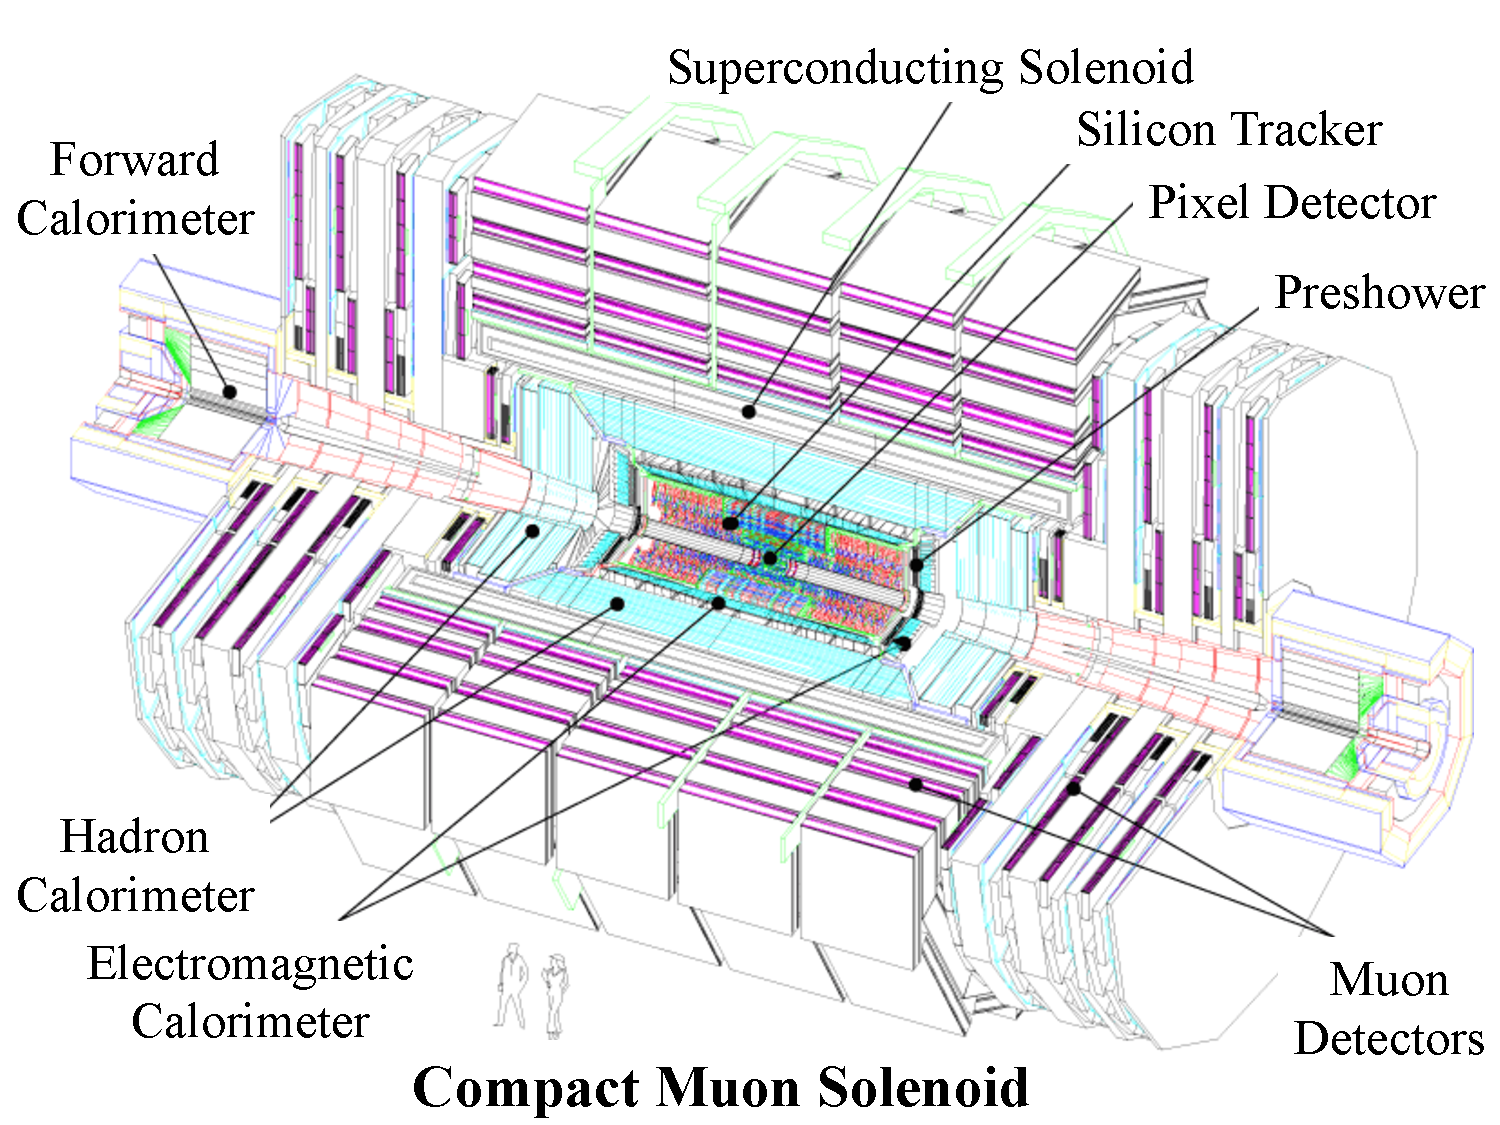
\includegraphics[width=0.8\textwidth]{Figures/Detector/cms_labelled.pdf}
       \caption{Schematic of the CMS detector.
	}
   	\label{fig:CMS}
\end{figure}

%%%%%%%%%%%%%%%%%%%%%%%%%%%%

\section{Coordinate system}
\label{sec:coordinates}
The origin of the CMS detector coordinate system is located at the nominal collision point. The $z$-axis is oriented along the beam direction, with the positive $z$-axis pointing in the counter-clockwise direction when viewing the LHC from above. The $y$-axis points vertically upward, and the $x$-axis points toward the center of the LHC. The $xy$-plane is referred to as the transverse plane.

Due to the nature of particle collisions, however, Cartesian coordinates are often not the most convenient. Because protons are not elementary particles, it is actually the individual quarks or gluons within the proton that interact during the collision. This means that the collision will not be at rest in the lab frame, but will have some non-zero velocity along the $z$-axis. To deal with this, it is beneficial to use coordinates that are invariant under boosts in the $z$ direction. CMS follows the particle physics convention of describing the position of a particle in terms of its transverse momentum, azimuthal angle, and pseudorapidity. The transverse momentum \pt is defined as the magnitude of the momentum in the $xy$ plane. The azimuthal angle $\phi$ is defined in the transverse plane, with $\phi  = 0$ corresponding to the positive $x$-axis. Finally, the pseudorapidity is defined as $\eta = -\ln{\tan{ (\theta / 2 )} } $, where the polar angle $\theta$ is measured from the $z$-axis. 

%%%%%%%%%%%%%%%%%%%%%%%%%%%%

\section{Superconducting solenoid}
\label{sec:magnet}

One of the most important components of the CMS detector is the superconducting solenoid that provides the bending power necessary to precisely measure the momentum of all charged particles produced in the collision. The solenoid is a 4-layer niobium-titanium coil embedded in aluminum and aluminum alloy. The magnet is located between the calorimeters and the muon system. It is 12.5 m long and has an inner diameter of 6 m. It is capable of producing magnetic fields up to 4 T, although the magnet is generally operated at 3.8 T to prolong its lifetime. At full current, the magnet has a stored energy of 2.6~GJ. A 12,000 ton steel yoke made up of 5 wheels in the barrel and 3 endcap disks serves to return the magnetic flux. The solenoid is suspended in a vacuum cryostat and cooled to 4.5K with liquid helium. A detailed description of the CMS magnet can be found in~\cite{magnetTDR}. Figure~\ref{fig:magnet} shows the calculated magnetic field in a longitudinal slice of the CMS detector.

\begin{figure*}[h!]
	\centering
	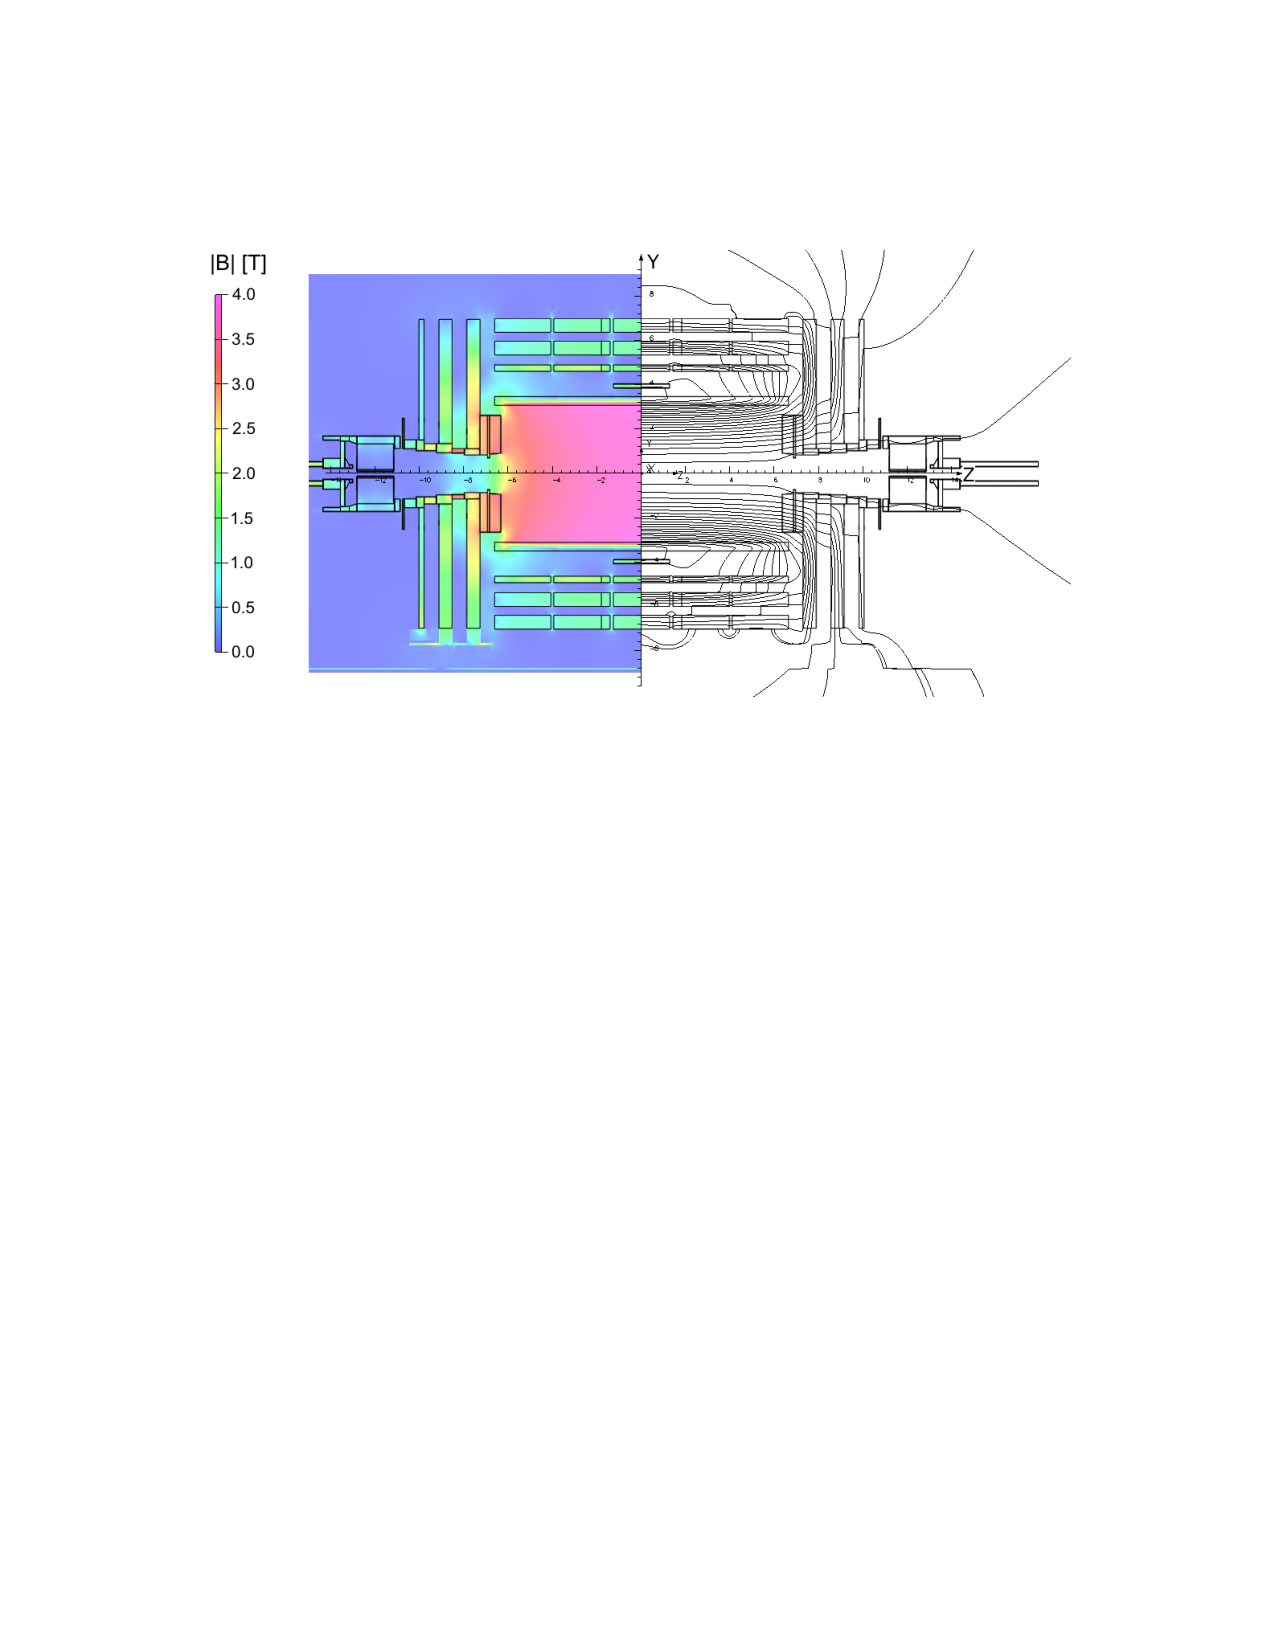
\includegraphics[width=\linewidth]{Figures/Detector/magnet.pdf}
       \caption{Calculated magnetic field $|\vec{B}|$ for a longitudinal slice of the CMS detector when operated at a central magnetic flux density of 3.8 T. In the right-hand portion of the figure, each magnetic field line represents a magnetic flux step of 6 Wb. Reprinted from Reference~\cite{CMSMagnetField}.}
       \label{fig:magnet}
\end{figure*}

%%%%%%%%%%%%%%%%%%%%%%%%%%%%

\section{Tracker}
\label{sec:Tracker}

The innermost sub-detector is the silicon tracker~\cite{trackerTDR,trackerTDRAddendum}. The tracker must provide enough information to accurately reconstruct the trajectories of charged particles to a high level of precision. This is accomplished through the use of silicon semiconductors, which rely on the properties of p-n junctions to detect charged particles. A p-n junction is created by bringing a p-type semiconductor into contact with an n-type semiconductor. For p- and n-type semiconductors, the crystal lattice of the semiconductor is doped to either donate or accept extra electrons, respectively. In a p-n junction, the extra electrons in the n-type semiconductor migrate and combine with the electron holes in the p-type semiconductor. This creates a depletion region in the center of the sensor. Charged particles moving through the depletion region will create electron-hole pairs that move towards either end of the junction. The resulting current is proportional to the energy deposited in the detector.

The overall dimensions of the tracker are 5.6 m long and 1.2 m in radius. The full tracking system is cylindrical in shape and is comprised of a barrel and two endcaps, each of which is split into layers of silicon pixel detectors and layers of silicon micro-strip detectors. In total, there are 48 million $150\times100~\mu$m pixels and 9.6 million strips that are between 80 and 180 $\mu$m wide. Figure~\ref{fig:TrackerLayout} shows a schematic drawing of the layout of the tracker subsystems. For charged hadrons with transverse momentum \pt less than 20 GeV, the \pt can be measured with a resolution of $1\%$. 

\begin{figure*}[h!]
	\centering
	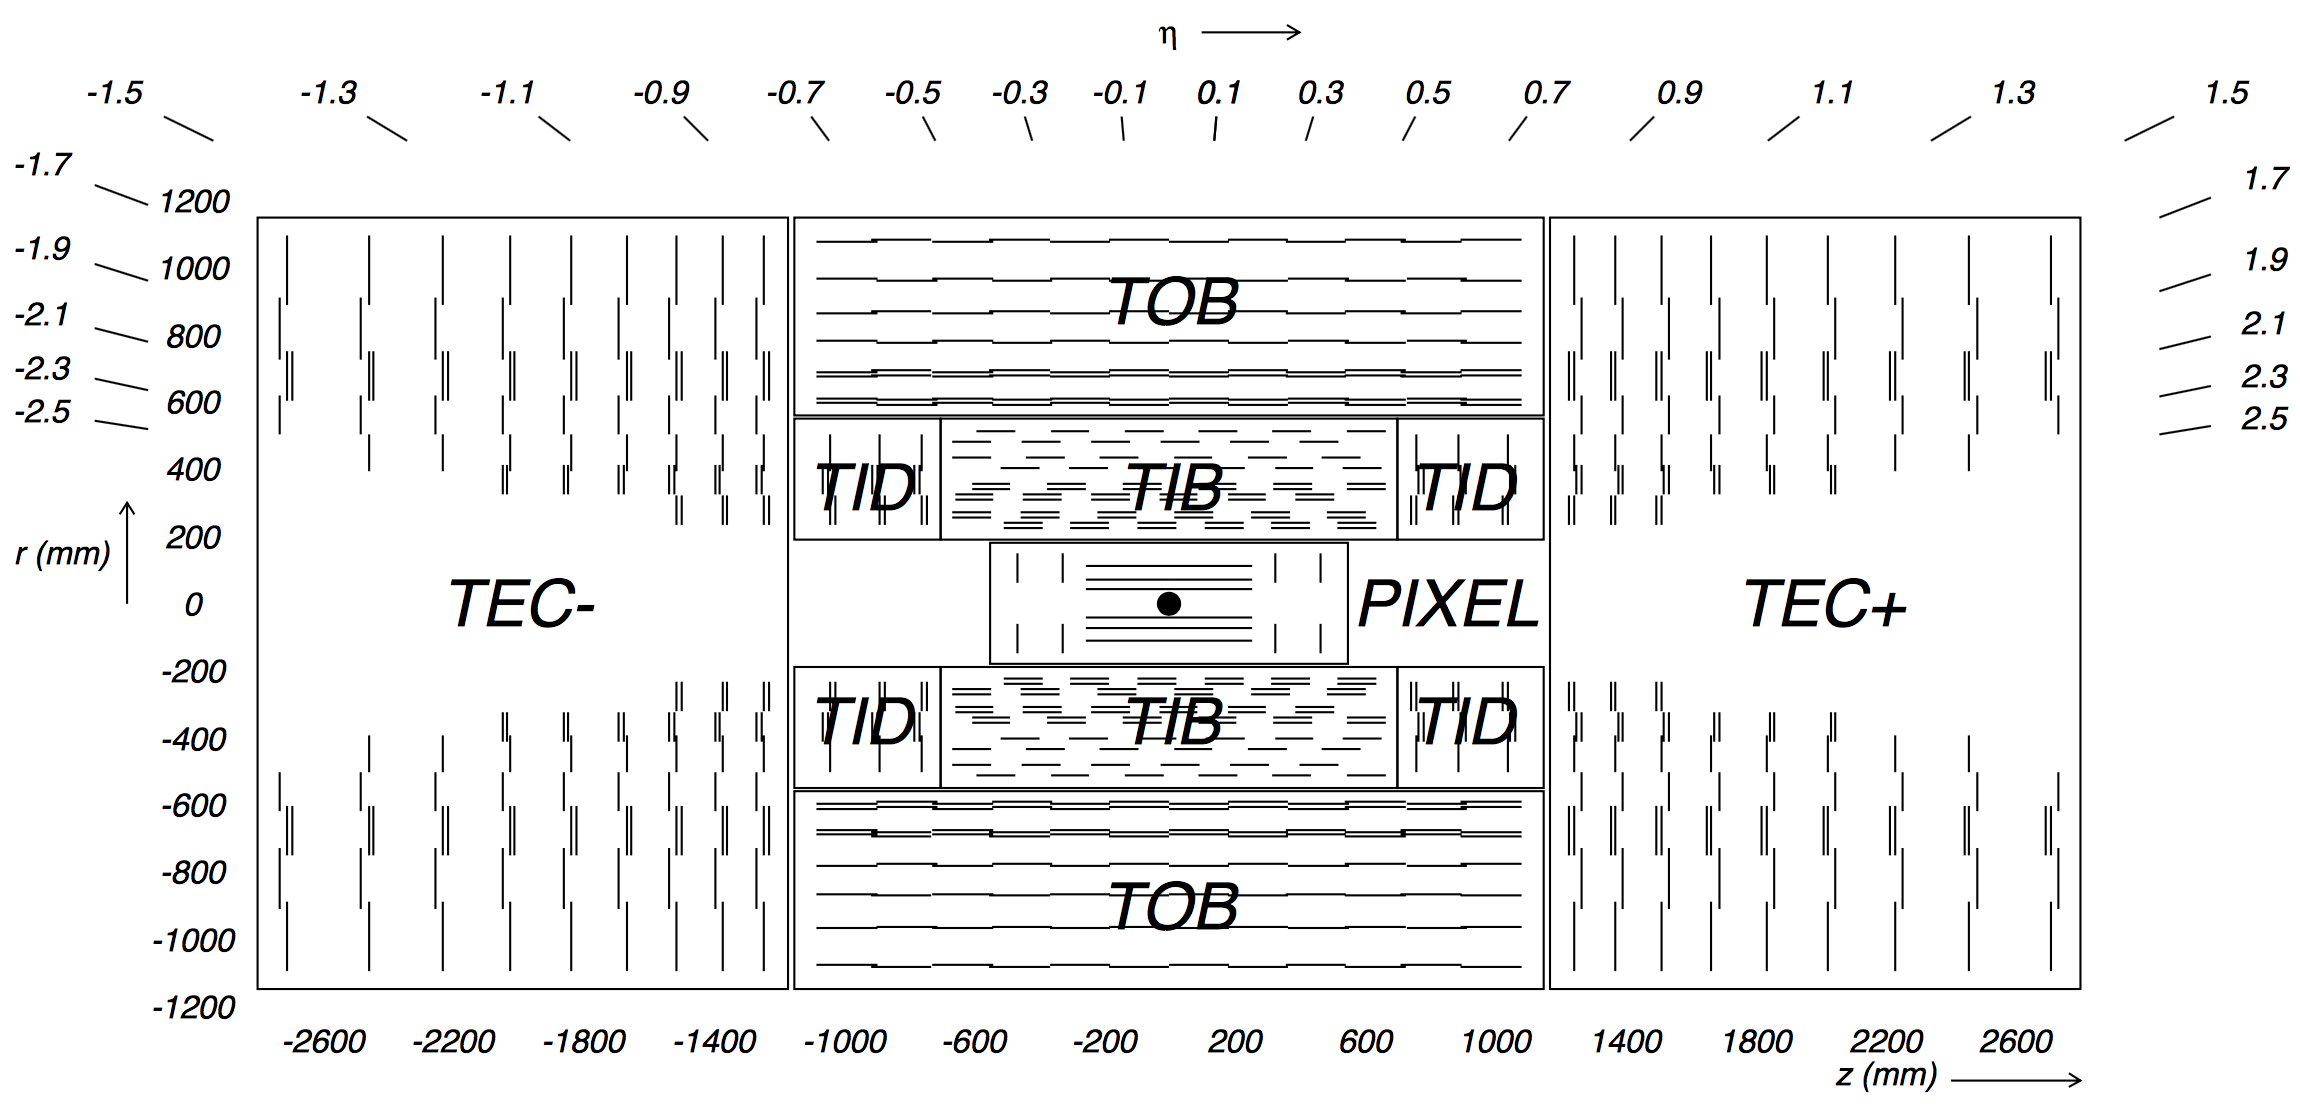
\includegraphics[width=\linewidth]{Figures/Detector/tracker_layout.png}
       \caption{Schematic of the CMS tracker system. Detector modules are represented by single lines, and back-to-back modules are represented by double lines. The strip tracker is further divided into the Tracker Inner/Outer Barrel (TIB/TOB), Tracker Inner Disk (TID) and the Tracker Endcap (TED). Reprinted from Reference~\cite{Chatrchyan2008zzk}.}
   	\label{fig:TrackerLayout}
\end{figure*}

\subsection{Pixel detector}
\label{sec:TrackerPixel}

Due to the high occupancy of the tracker within 10 cm of the beam pipe, pixel detectors rather than strip detectors are used as the innermost layers of the tracker. Three layers in the barrel and two disks of pixel detectors in the endcap give three high-precision points for every charged particle moving away from the interaction point. The small pixel size of $150\times100~\mu$m is critical for accurate secondary vertex reconstruction, for forming seed tracks used for high level triggering (see Chapter~\ref{chap:Trigger}), and for the reconstruction of charged particles in the event (see Chapter~\ref{sec:EventReconstruction}). The three barrel layers are 53 cm long and are located at mean radii of 4.4, 7.3 and 10.2 cm. The endcap modules extend radially from 6 to 15 cm and are placed on each side at $z=\pm34.5$ and $z=\pm46.5$~cm. The endcaps extend the coverage of the sub-detector to $|\eta|~<~ 2.5$. 
%Yutaro: An interpolation of the signal amplitudes gives a spacial resolution of 15-20 mum, (because charge is shared between several pixels due to the geometry and the magnetic field)

\subsection{Strip detectors}
\label{sec:TrackStrip}
Moving radially beyond the pixel detectors are the silicon strip trackers. These operate on the same basic principles as the pixel detectors, but each silicon strip is 10 cm $\times~80~\mu$m, giving a precise position measurement along one dimension only. In the barrel, the strips run parallel to the $z$-axis with a pitch, or spacing between strips, between 80 and 183 $\mu$m. Strips in the endcaps are aligned radially with a pitch between 100 and 184 $\mu$m. In total there are 10 layers of strip sensors in the barrel and 12 layers in the endcaps.

The tracker has a spatial resolution of 25-50 $\mu$m perpendicular to the strip direction. In order to improve the precision of the detector in the direction parallel to the strips, several of the layers are arranged in pairs. By aligning the second layer 100 mrad off from the strips in the first layer, a spatial resolution of 230 to 530 $\mu$m can be achieved. These back-to-back modules are represented by double lines in Figure~\ref{fig:TrackerLayout}.

%Yutaro: paragraph on the alignment system for the strips.

%%%%%%%%%%%%%%%%%%%%%%%%%%%%

\section{Electromagnetic Calorimeter (ECAL)}
\label{sec:ECAL}

Very important. Finds photons.


%%%%%%%%%%%%%%%%%%%%%%%%%%%%

\section{Hadron calorimeter (HCAL)}
\label{sec:HCAL}

brass sampling calorimeter

%%%%%%%%%%%%%%%%%%%%%%%%%%%%

\section{Muon system}
\label{sec:Muon}

The muon subsystem is located outside of the solenoid and is embedded in the return yoke for the magnetic flux. Three different types of detectors are used in the muon system: drift tube chambers (DTC) = positively charged wire within gas volume. Muon knocks electrons off atoms in the gas, which are attracted to the wire. Can determine where electrons hit and where the muon was from the wire to get 2 coordinates for its position. Barrel
Cathode strip chamber (CSC) = better for high flux areas. Crisscrossing positive and negative wires. Muons knock off electrons, which go to positive wires. Ions move toward negative wires. Two position coordinates. Endcaps.


